\subsection{Classifier: Diagonal Covariance (Per-Class)}

% \begin{figure}[H]
%     \centering
%     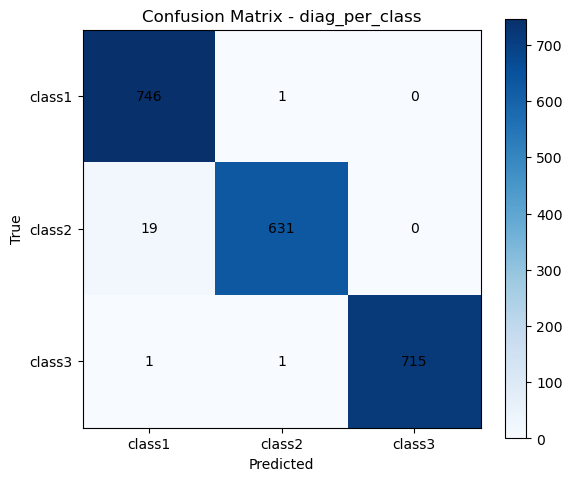
\includegraphics[width=0.75\linewidth]{images/RD_Group04_images/03_diag_per_class/01_confusion_matrix.png}
%     \caption{Confusion Matrix for Diagonal Covariance (Per-Class) (Vowel Data)}
% \end{figure}

\begin{table}[H]
\centering
\caption{Confusion Matrix for Diagonal Covariance (Per-Class) (Vowel Data)}
\label{tab:confmat_d3_sigma2I}
\begin{tabular}{|c|c|c|c|}
\hline
\textbf{Actual $\backslash$ Predicted} & \textbf{Class 1} & \textbf{Class 2} & \textbf{Class 3} \\
\hline
\textbf{Class 1} & 746 & 1   & 0   \\
\textbf{Class 2} & 19  & 631 & 0   \\
\textbf{Class 3} & 1   & 1   & 715 \\
\hline
\end{tabular}
\end{table}

\begin{table}[H]
\centering
\caption{Performance Metrics - Diagonal Covariance (Per-Class)}
\begin{tabular}{lcccc}
\toprule
\textbf{Class} & \textbf{Precision} & \textbf{Recall} & \textbf{F1-Score} & \textbf{Support} \\
\midrule
Class 1 & 0.9739 & 0.9987 & 0.9861 & 747 \\
Class 2 & 0.9968 & 0.9708 & 0.9836 & 650 \\
Class 3 & 1.0000 & 0.9972 & 0.9986 & 717 \\
\midrule
\textbf{Accuracy} & \multicolumn{4}{c}{0.9896} \\
\textbf{Mean Precision} & \multicolumn{4}{c}{0.9902} \\
\textbf{Mean Recall} & \multicolumn{4}{c}{0.9889} \\
\textbf{Mean F1 Score} & \multicolumn{4}{c}{0.9895} \\
\bottomrule
\end{tabular}
\end{table}

\textbf{Inferences:} Axis-aligned ellipses fit the data well. Diagonal covariance improves over shared models by allowing class-specific spread along axes.

\begin{figure}[H]
    \centering
    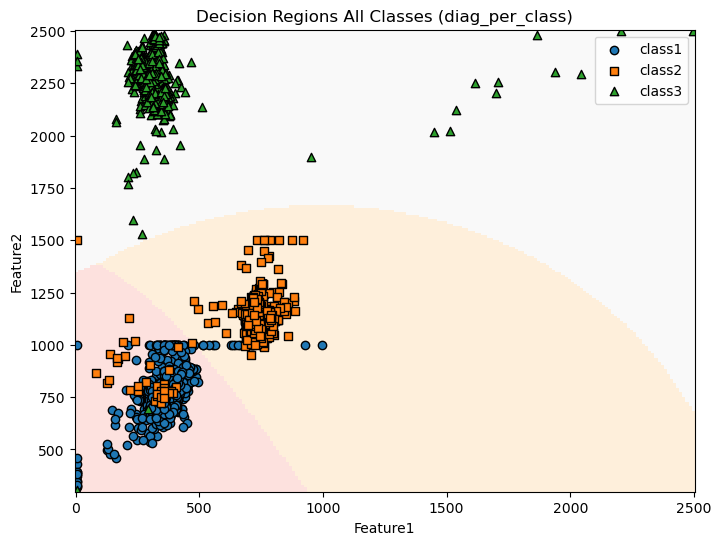
\includegraphics[width=0.85\linewidth]{images/RD_Group04_images/03_diag_per_class/05_decision_region_all.png}
    \caption{Decision Region Plot (All Classes) - Diagonal Covariance (Per-Class)}
\end{figure}

\subsubsection{Decision Region Plots Between Class Pairs (RD Dataset, Diagonal Covariance (Per-Class)}

\begin{figure}[H]
    \centering
    \begin{minipage}{0.32\linewidth}
        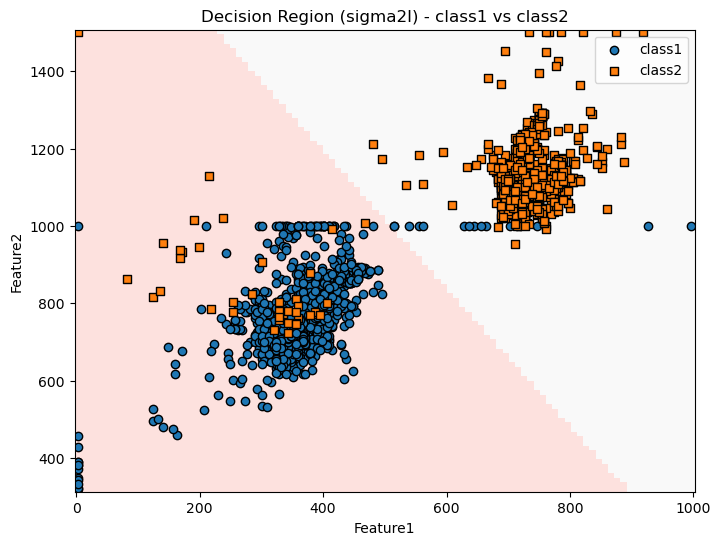
\includegraphics[width=\linewidth]{images/RD_Group04_images/01_sigma2i/02_decision_region_c1_c2.png}
        \caption*{Class 1 vs Class 2}
    \end{minipage}
    \hfill
    \begin{minipage}{0.32\linewidth}
        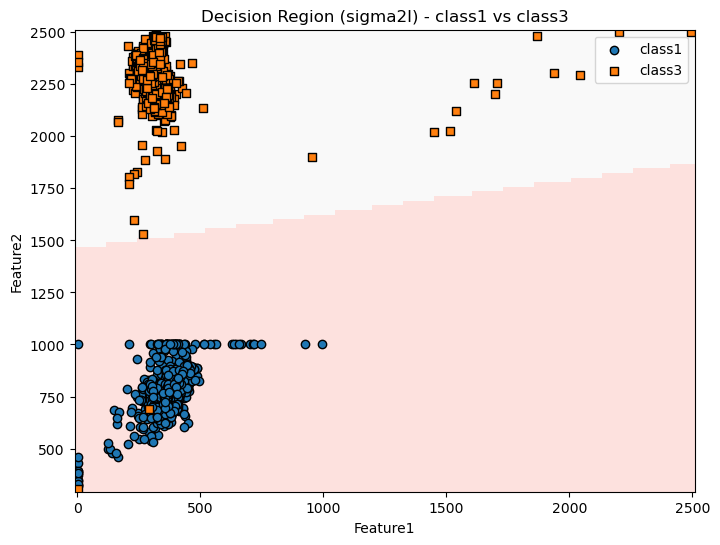
\includegraphics[width=\linewidth]{images/RD_Group04_images/01_sigma2i/03_decision_region_c1_c3.png}
        \caption*{Class 1 vs Class 3}
    \end{minipage}
    \hfill
    \begin{minipage}{0.32\linewidth}
        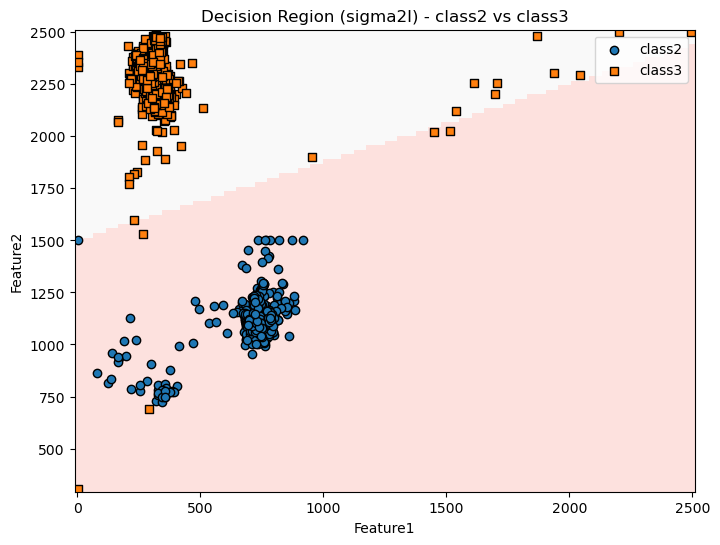
\includegraphics[width=\linewidth]{images/RD_Group04_images/01_sigma2i/04_decision_region_c2_c3.png}
        \caption*{Class 2 vs Class 3}
    \end{minipage}
    \caption{Decision Region Plots (Training data points superimposed) between class pairs for Diagonal Covariance (Per-Class) on RD dataset}
\end{figure}